\documentclass[aspectratio=169]{beamer}

\mode<presentation>
{
  \usetheme{default}
  \usecolortheme{default}
  \usefonttheme{default}
  \setbeamertemplate{navigation symbols}{}
  \setbeamertemplate{caption}[numbered]
  \setbeamertemplate{footline}[frame number]  % or "page number"
  \setbeamercolor{frametitle}{fg=white}
  \setbeamercolor{footline}{fg=black}
} 

\usepackage[english]{babel}
\usepackage[utf8x]{inputenc}
\usepackage{tikz}
\usepackage{courier}
\usepackage{array}
\usepackage{bold-extra}
\usepackage{minted}
\usepackage[thicklines]{cancel}

\xdefinecolor{dianablue}{rgb}{0.18,0.24,0.31}
\xdefinecolor{darkblue}{rgb}{0.1,0.1,0.7}
\xdefinecolor{darkgreen}{rgb}{0,0.5,0}
\xdefinecolor{darkgrey}{rgb}{0.35,0.35,0.35}
\xdefinecolor{darkorange}{rgb}{0.8,0.5,0}
\xdefinecolor{darkred}{rgb}{0.7,0,0}
\definecolor{darkgreen}{rgb}{0,0.6,0}
\definecolor{mauve}{rgb}{0.58,0,0.82}

\title[2018-02-28-iml-uproot]{\vspace{0.5 cm} \\ 
\includegraphics[width=0.25\linewidth]{uproot-logo.pdf} \\ Rapidly moving data from ROOT to Numpy and Pandas}
\author{Jim Pivarski}
\institute{Princeton University -- DIANA-HEP}
\date{February 28, 2018}

\begin{document}

\logo{\pgfputat{\pgfxy(0.11, 7.4)}{\pgfbox[right,base]{\tikz{\filldraw[fill=dianablue, draw=none] (0 cm, 0 cm) rectangle (50 cm, 1 cm);}\mbox{\hspace{-8 cm}
\includegraphics[height=1 cm]{princeton-logo-long.png}
\includegraphics[height=1 cm]{diana-hep-logo-long.png}}}}}

\begin{frame}
  \titlepage
\end{frame}

\logo{\pgfputat{\pgfxy(0.11, 7.4)}{\pgfbox[right,base]{\tikz{\filldraw[fill=dianablue, draw=none] (0 cm, 0 cm) rectangle (50 cm, 1 cm);}\mbox{\hspace{-8 cm}
\includegraphics[height=1 cm]{princeton-logo.png}
\includegraphics[height=1 cm]{diana-hep-logo.png}}}}}

% Uncomment these lines for an automatically generated outline.
%\begin{frame}{Outline}
%  \tableofcontents
%\end{frame}

% START START START START START START START START START START START START START

\begin{frame}{The what and why of uproot}
\vspace{0.5 cm}

\begin{block}{What is uproot?}
A pure Python $+$ Numpy implementation of ROOT I/O.
\end{block}

\vspace{0.5 cm}
\begin{block}{Why does it exist?}
\begin{enumerate}
\item To extract columnar data (branches) from a ROOT file without invoking the event-handling infrastructure of the ROOT framework.
\item As a faster and fewer-dependencies alternative to root\_numpy and root\_pandas.
\item To express the semantics and conventions of the ROOT file format independently of ROOT, in lieu of a formal specification.
\end{enumerate}
\end{block}
\end{frame}

\begin{frame}{Multiple implementations of the same format?}
\vspace{0.25 cm}
\begin{columns}
\column{0.73\linewidth}
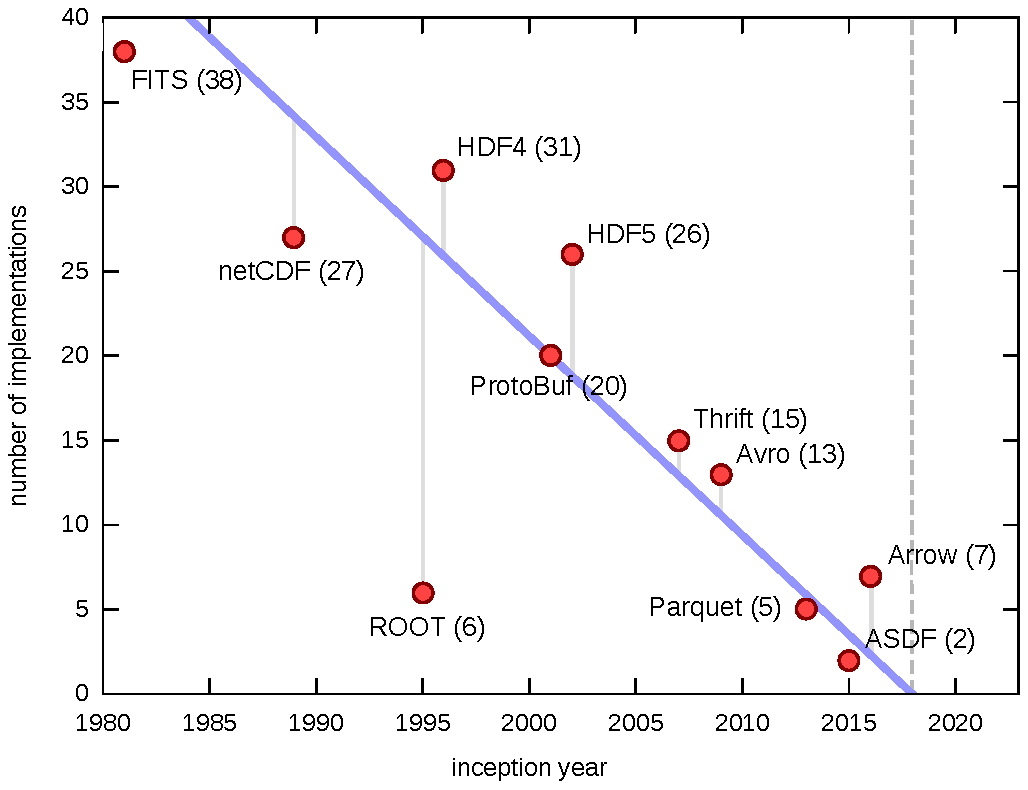
\includegraphics[width=\linewidth]{formats.pdf}
\column{0.25\linewidth}
It's more common to define a specification and implement many interpreters than not.

\vspace{0.25 cm}
Most connect the format to different contexts, such as different languages.

\vspace{0.25 cm}
\small\textcolor{gray}{(Take these numbers with a grain of salt: HDF5 is {\it criticized} because many of its bindings depend on only two C libraries!)}
\end{columns}
\end{frame}

\begin{frame}{ROOT I/O implementations}
\vspace{0.25 cm}
\begin{columns}
\column{1.2\linewidth}
\renewcommand{\arraystretch}{1.6}
\begin{tabular}{p{2.4 cm} c p{4.7 cm} p{5.25 cm}}
\centering ROOT & C++ & ROOT itself & The ROOT Team \\
\centering FreeHEP I/O $\to$ spark-root & Java/Scala & For Spark and other Big Data projects that run on Java & Started by Tony Johnson in 2001, updated by Viktor Khristenko \\
\centering RIO $\to$ inlib/exlib & C++ & Intended as an alternative, now embedded in GEANT-4 & Guy Barrand \\
\centering JsRoot & Javascript & For interacting with ROOT in web browsers or standalone & Bertrand Bellenot, Sergey Linev (in the ROOT Team) \\
\centering go-hep/rootio & Go & HEP analysis ecosystem in Go & Sebastien Binet \\
\centering \textcolor{blue}{uproot} & \textcolor{blue}{Python} & \textcolor{blue}{For quickly getting ROOT data into Numpy and Pandas for machine learning} & \textcolor{blue}{Jim Pivarski (me)} \\
alice-rs/root-io & Rust & ALICE ecosystem in Rust & Christian Bourjau \\
\end{tabular}
\end{columns}
\end{frame}

\begin{frame}{Why Python $+$ Numpy?}
\vspace{0.25 cm}
\begin{itemize}\setlength{\itemsep}{0.35 cm}
\item Physicists are already using Python for data analysis.

\begin{itemize}
\item \textcolor{gray}{PyROOT has excellent coverage of the ROOT ecosystem. However, calling individually wrapped C++ methods from Python is slow and the two languages have different (often conflicting) memory management.}

\item \textcolor{gray}{Performance-oriented tools like root\_numpy and root\_pandas compile into a specific version of ROOT, which complicates upgrades. Also, asking for arrays through interfaces designed for event processing is a severe performance penalty.}
\end{itemize}

\item The scientific Python ecosystem, including much of machine learning, is designed around a fundamental abstraction called the Numpy array.

\item Working with computer scientists is easier when you can say, ``pip install uproot.''

\item Implemented correctly, Python $+$ Numpy doesn't have to be slow.

\begin{itemize}
\item \textcolor{gray}{Finding the columnar data in a ROOT file may be done in slow Python, as long as decompression and array manipulations are done by compiled code.}
\end{itemize}
\end{itemize}
\end{frame}


\end{document}
